\chapter{\etherbase: Improving Reproducibility in Smart Contract Research} \label{ch:etherbase}


\section{Introductory Remarks}
	\label{sec:intro}
	Ethereum is the most widely used blockchain platform with millions of smart contracts written on it, with a market cap of over 250 billion U.S. Dollars.
	Simply put, a smart contract is a self-exeucting program stored on the Ethereum blockchain that runs when pre-defined conditions are satisfied.
	The research community in the past few years has put in the effort to develop automated analysis tools and frameorks~\cite{ref_tools} that locate and eliminate vulnerabilities in smart contracts for the purposes of making smart contracts more secure as their adoption is ever increasing in different sectors of decentralized finance..
	In a study in 2020, researchers analyzed about one million Ethereum smart contracts and found 34,200 of them to be potentially vulnerable.~\cite{ref_flag1}
	Another research effort showed that 8,833 (around \%46) smart contracts on the Ethereum blockchain were flagged as vulnerable out of 19,366 smart contracts.~\cite{ref_flag2}, ~\cite{Empirical-Evaluation-of-Smart-Contract-Testing:What-is-the-Best-Choice}

	Comparing and reproducing such research is not an effortless process.~\cite{Empirical-Evaluation-of-Smart-Contract-Testing:What-is-the-Best-Choice}
	Most of the datasets used to test and benchmark those very same tools proposed in the research literature are not publicly or easily available to the research community.
	This makes reproduction efforts immensely hard and and time-intensive to carry out.

	The current approach to compare one's tools / methodologies of evaluating the security of smart contracts with that of another researcher / toolset,
	is to make do with whatever out-of-date incomprehensive and unrepresentative dataset they have at their disposal, a very timely and inefficient process.
	In other cases, the researchers need to start from scratch and create their own datasets, a non-trivial and slow process.
	What makes it worse is the data bias, which can be introduced in a dataset in different phases of data acquisition and data cleaning.
	This can easily escalate to become a threat to validity in the research.~\cite{Empirical-Evaluation-of-Smart-Contract-Testing:What-is-the-Best-Choice}

	In this chapter, we present \etherbase, an extensible, and queryable database that facilitates and enhances the verification and reproducibility of previous empirical
	research and lays the groundwork for faster, more rapid production of research on smart contracts.
	\etherbase~is open-source and publicly available.
	The source code for data acquisiton and cleaning is not available due to private IP reasons, and only the collected data and the database is accessibel to the public.
	Researchers, smart contract developers, and blockchain-centric teams and enterprises can also use such corpus for specific use-cases.

	In summary, we make the following contributions with \etherbase.
	\begin{enumerate}
		\item We propose \etherbase, a systemic and up-to-date database for Ethereum by exploiting its intetrnal mechanisms.
		\item We implement \etherbase and make its pipelines open-source. It obtains historical data and facilitates benchamrking and reproduction in research and development for new toolsets. It is more up-to-date than existing datasets, gets sutomatically reviewed and renewed, in comparison to the previous manual one-time data gathering efforts.
		\item We propose the first dataset of Ethereum smart contracts which has a mix of off-chain and on-chain data together, meaning that it contains the source code and the bytecode of
		the corresponding smart contracts in the same dataset.
		\item We propose the first automatically up-to-date laballed dataset of Ethereum smart contracts with vulnrabilities.
	\end{enumerate}

\section{Related Work}
	\label{sec:relwork}
	We assume the reader is familiar with blockchain technology, Ethereum blockchain, and its primary high-level programming language Solidity.
	Ethereum Smart contracts are developed mostly in the programming language Solidity and for execution, they get compiled to their corresponding bytecode.
	EVM takes bytecode as input and works in a stack-based architecture with a word size of 256 bits.
	There are three different spaces in EVM to store data and resources, namely stack, memory and storage.~\cite{liu2019enabling}
	In this section we present and discuss references and information for some of the more prominent publicly available smart contract benchamrk datasets which were identified in our studies.

	SmartBugs~\cite{Empirical-Review-of-Automated-Analysis-Tools-on-47587-Ethereum-Smart-Contracts} makes the top of the list as one of the most used benchmarks in the research space.
	In this work, Durieux et al. presented an extensible and easy-to-use execution framework for benchmarking different security analysis tools for Ethereum smart contracts.
	They empirically evaluated 9 analysis tools on a small (< 100)labelled  dataset of vulnerabilities.
	Ren et al. provide a dataset consisting of 47,518 un-annotated smart contracts with the history of at least one executed transaction on the blockchain.
	For researchers trying to build upon such work, using the unlabelled dataset is a great improvement for both tool development and reproduction efforts, but because of the lack of some degree of ground truth in the dataset, it's not possible to easily apply, for example, supervised amchine learnign algorithms to that dataset.
	Their labeled dataset contains about a thousand smart contracts which is good for initial benchmarkings, but it only the source code of the contracts are available and does not provide any bytecode for them.

	Ren et al.~\cite{Empirical-Evaluation-of-Smart-Contract-Testing:What-is-the-Best-Choice} created a benchmark suite that integrates annotated and unlabelled raw smart contracts from a variety of sources
	such as Etherscan~\cite{etherscan}, SolidiFI repository, CVE Library, and Smart Contract Weakness (SWC) Registry.
	They collected 45,622 real-world diversified Ethereum smart contracts and proposed a systematic evaluation process and performed extensive experiments.
	Their labeled dataset has 350 manually generated contracts.

	Many of the authors of the tools proposed in this practice leverage unlabelled datasets to evaluate the performance of their toolset.
	The publicly available datasets are either not appropriately annotated or a very small subset of them is labelled with the vulnerabilities's identification properties.
	This is because the number of the contracts -most of them being clones of other smart contracts- is so huge, they cannot be all manually annotated.
	To the best of our knowledge, there has been only one annotated dataset, realeased publicly, from Yashavant et al.~\cite{yashavant2022scrawld}
	We strive to build upon that work and make facilitate the processes of reproduction in the smart contract research community.
	Our dataset has the advantage of updating regularly, and being more comprehensive with the more updated Solidity versions of different smart contracts available in the dataset.

	Kalra et al.~\cite{kalra2018zeus} published their analysis results for 1,524 smart contracts with no other information or metadata in relation to those contracts.

	Luu et al.~\cite{oyente} collected 19,366 smart contracts from the blockchain and provided their blockchain addresses alongside analysis results on each contract on whether they contain any of their selected four vulnerabilitis or not.

	In 2022, Yashavant et al. ~\cite{yashavant2022scrawld}

	The smart contract source codes collected in GitHub repositories associated with the previously published literature do not directly reference smart contracts deployed on the blockchain through an Ethereum address;~\cite{pierro2020organized}
	this makes it hard to determine if the identified smart contracts have been tested or used on the Ethereum blockchain or not.
	GitHub repositories of the available datasets do not implement a search engine or query capability to filter smart contracts based on particular
	metrics or parameters, such as the ETH value or the number of internal transactions for a smart contract.
	
	The GitHub repositories related to the published literature usually only provide the raw datat of the smart contracts without any proper documentation, comments, or further annotations on the data connected to the collected smart contracts.
	None of the GitHub repositories currently available to the public or used in research papers provide smart contract ABI's or Opcodes to the best of our knowledge.
	
	As a user of the Website Etherscan, you can easily search the Ethereum blockchain for any specific smart contract given the availability of its address but when it comes to downloading the data
	for that smart contract or any other batch of smart contracts,  using Etherscan has its limits:~\cite{pierro2020organized}:
	Smart contracts' data is massive, based on the estimation from ~\cite{pierro2020organized},
	and the daily limits on the API's provided by Etherscan make retrieving that data even harder.
	The API provided by Etherscan does not allow the users to obtain a list of the addresses of their desired smart contracts.
	The  API calls currently available only allow navigation at the block-level.
	A researcher cannot easily explore the source code for their collected smart contracts.
	First, they would have to to inspect any block on-chain and then search for any transactions that have a receive/send address associated with that specific smart contract.

\section{Methodology}

	\begin{figure}[t]
		\centering
		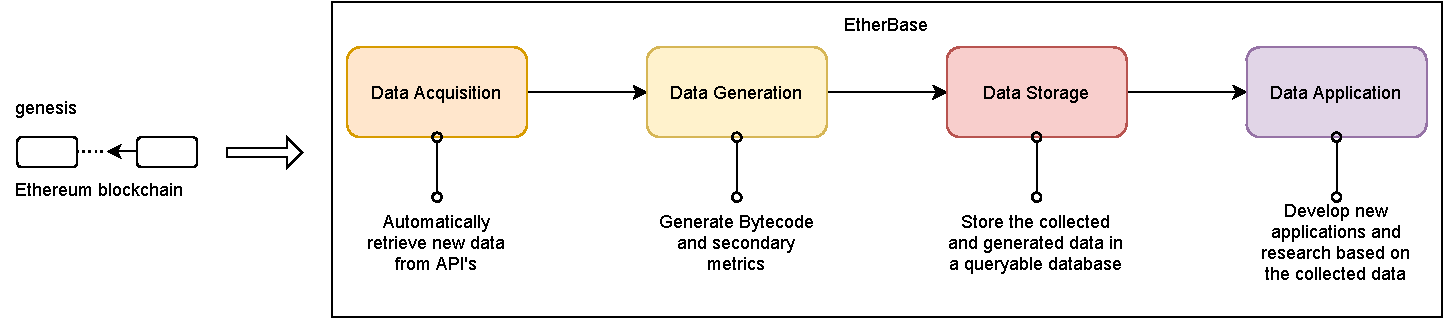
\includegraphics[width=1\textwidth]{figures/Untitled Diagram.pdf}
		\caption{EtherBase Worflow}
		\label{fig:my_label}
	\end{figure}
	
	We specifically designed \etherbase to not provide the end-users with a dump of contracts and their corresponding features in a vague file hierarchy.
	We have a service offering the ability to filter and analyze smart contracts and a dataset of smart contracts with interesting features to conduct empirical research on, according to metrics like Pragma version, ETH value, etc.
	To fulfill its purpose, \etherbase is designed to perform four primary automatic operations on the data:
	\begin{enumerate}
		\item \textbf{Data Acquisiton}: Automatic retrieval of off-chain and on-chain data
		\item \textbf{Data Generation}: Generation of bytecode and other metrics
		\item \textbf{Data Storage}: Storage of the collected data in a public and accessible way
		\item \textbf{Data Application}: Development of new applications and research based on the available database
	\end{enumerate}

	The next sections walk through the above-mentioned steps of the workflow one-by one.

	\subsection{Data Acquisition}
		The current dataset corresponds to the contracts collected from Etherscan, the most used service for researchers trying to collected smart contracts from the Ethereum blockchain.
		Every contract stored on Etherscan's database is indexed by its own corresponding addresses,
		In order to collect the contracts, we retrieve the addresses for every contract which has more than one transaction through Google BigQuery, like the process done by ~\cite{Empirical-Evaluation-of-Smart-Contract-Testing:What-is-the-Best-Choice}.
		Using Google BigQuery query request service, we obtain 1,712,347 distinct contract addresses that have more than one transactions associated with them.

	\subsection{Data Generation}
		Instead of manually writing scripts to obtain the source code, bytecode, and other metadata via services like Etherscan, we leverage a tool designed and maintained by Trail of Bits, namely Cyitic-compile.
		All the previous works of research, work on providing either source code or bytecode of smart contracts to the researchers, but that will not be enough for the users who want to compile the smart contracts or build tools upon such data.
		Compiling smart contracts is also a tricky busines, due to the rapid pace of changing versions of the dominant programming language, Solidity, used to write and develop smart contracts.
		We developed crytic-compile, a library to help the compilation of smart contracts, to help with this problem.
		It helps the user to be needless of maintaining an interface with solc and it automatically finds and uses the right version of solc or a better compatiable version of solc to compile the input smart contracts.
		They way this works under the hood is that crytic-compile compiles an input smart contract and outputs a compilation untit in the standard solc output format, written in a json file, alongside the source code and other metadata.
		Unlike the other proposed datasets and tools discussed in Section~\ref{sec:relwork}, EtherBase targets the core problem of the lack of reproducibility in the research literature.
		Discussions surrounding what types of secondary metrics to retrieve from the Ethereum blockchain or third-party services will be explored further.
		
		For the rest of the analysis of the collected contracts, we only get to work on contracts with available source-code.
		We adopt the method used in the work of ~\cite{deduplicate} to remove the duplicates smart contracts,
		that is checking the MD5 checksums of each of the two source files in the collected dataset to see if they are the same and after removing the whitespace among the lines of code.
		After the process of deduplication is done, we get down to 48,622 smart contracts contracts.
		For this paper and as of now, we have released 5,000 smart contracts for the tool comparison purposes.
		There exist many metrics that we have access to, can calculate, and add to \etherbase, but not a lot of research has been conducted on the applicability
		of these many different types of metrics to empirical research on the Ethereum blockchain or how much it appeals to the researchers active in this field.
		In the following, we describe the initial set of the metrics we selected to include in EtherBase in the form of a table, to be followed by more,
		after more discussion and research on their applicability to research on smart contracts.

		The built-in metrics relating to smart contracts are those features which depend on the internal properties of a smart contract, e.g. SLOC (Source Lines of Code), Pragma version, number of modifiers, payable, etc. Hence the title \emph{primary metrics}.

		For this table, we decided to include the core metrics of a smart contract, which would help a researcher collect a large set of smart contracts rapidly, and conduct further analysis on them, comprising of:

		\begin{table}[H]
			\caption{Primary Metrics on Smart Contracts}
			\label{tab:intrinsic-cues}
			\centering
			\begin{adjustbox}{width=1\textwidth}
			\def\arraystretch{1.3}
			\begin{tabular}{l|p{105mm}}
				\textbf{Name} & \textbf{Description} \\
				\hline
				\verb|Pragma| & The \verb|pragma| keyword is used to enable certain compiler features or checks.~\cite{pragmadocs}\\
				\verb|Contract Address| & Unique 20-byte address, used as the main index to distinguish smart contracts from each other. \\
				\verb|Creator Address| & Indicates the address of the deeployer of the smart contract. \\
				\verb|Source Code| & Source code of the smart contract, specific to the programming language Solidity. \\
				\verb|Bytecode (bin)| & . \\
				\verb|Bytcode (bin-runtime)| & . \\
				\verb|ABI| & The content of the application binary interface for each contract. \\
				\verb|Block Number| & The length of the blockchain in blocks. \\
				\verb|ETH Value| & The value of each smart contract in therms f=of the ETH thay hold. \\
				\verb|Transaction Count| & Number of internal transactions from eacch smart contract. \\
				%\verb|Deployer Status| & Indicates whether the deployer of a contract is a contract or not. \\
			\end{tabular}
			\end{adjustbox}
	\end{table}

	As for the primary metrics, here are our justifications for the above selection:

	\begin{itemize}

		\item{\verb|Pragma|: Source files can (and should) be annotated with a version pragma to halt compilation with future versions of Solc due to the possibility of introduction of incompatible changes with the version of the Solc used to write the original smart contract. Filtering through contracts via Pragma helps the researcher to collect a homogenuous set of contracts with a consistent synatx.}\\

		\item{\verb|Contract Address|: In Ethereum, the state is made up of objects called "accounts", with each account having a 20-byte address. Contract address is the main key in EtherBase for distinguishing contracts from each other.}\\

		\item{\verb|Creator Address|: The contract address is usually given when a contract is deployed to the Ethereum Blockchain. The address comes from the creator's address, where the contract has been initially deployed from, alongside the number of transactions sent from that address (the “nonce”). A creator's address can be helpful in analyzing the clone ratio and }\\

		\item{\verb|Source Code|: The source code of each Ethereum smart contract is written in Solidity and helps researchers do all sortds of analysis on the smart contracts.}\\

		\item{\verb|Bytecode (bin)|: The regular \verb|bin| output is the code placed on the blockchain plus the code needed to get this code placed on the blockchain, the code of the constructor.}\\

		\item{\verb|Bytecode (bin-runtime)|: \verb|bin-runtime| is the code that is actually placed on the blockchain.}\\

		\item{\verb|ABI|: \verb|ABI| stands for application binary interface. It's basically how you can encode Solidity contract calls for the EVM and, backwards, how to read the data out of transactions.}\\

		\item{\verb|Block Number|: \verb|Block Number|is the length of the blockchain in blocks, more specifically the block on which the smartt contract exists.}\\
		\item \verb|ETH Value|: The ETH every smart contract hols is an excellent filter or bar to select "interesting" contracts through for further research on the contracts that are more \emph{active} on the blockchain.\\

		\item \verb|Transaction Count|: Like ETH Value, transaction count is an important metric for us to be able to exclude contracts that do not participate much on the chain and hence, work on the contracts thast have a higher probability of interaction with more contracts.\\
		\end{itemize}
	
	\subsection{Data Storage}
			All of the smart contracts collected in the previous stage along with their corresponding metadata need to be stored somewhere and we choose a PostgreSQL database in the design, -alongside a GitHub repository- to make it easier for researchers and other users to manage, filter, and query their needed data.
			Afterwards and in the data application stage, users can analyse their queried data according their specific research queries.

			Figure 2 shows the directory structure of the collected data. The first leaf in the directory \texttt{Contracts} corresponds to the \\


\definecolor{folderbg}{RGB}{124,166,198}
\definecolor{folderborder}{RGB}{110,144,169}

\def\Size{4pt}
\tikzset{
  folder/.pic={
    \filldraw[draw=folderborder,top color=folderbg!50,bottom color=folderbg]
      (-1.05*\Size,0.2\Size+5pt) rectangle ++(.75*\Size,-0.2\Size-5pt);  
    \filldraw[draw=folderborder,top color=folderbg!50,bottom color=folderbg]
      (-1.15*\Size,-\Size) rectangle (1.15*\Size,\Size);
  }
}
\resizebox{0.6\textwidth}{!}{%
\begin{forest}
  for tree={
    font=\ttfamily,
    grow'=0,
    child anchor=west,
    parent anchor=south,
    anchor=west,
    calign=first,
    inner xsep=7pt,
    edge path={
      \noexpand\path [draw, \forestoption{edge}]
      (!u.south west) +(7.5pt,0) |- (.child anchor) pic {folder} \forestoption{edge label};
    },
    before typesetting nodes={
      if n=1
        {insert before={[,phantom]}}
        {}
    },
    fit=band,
    before computing xy={l=15pt},
  }  
[contracts
  [0
  ]
  [1
    [0
      [0
        [0
          [0
            [5
              [0x100005bc082d49eefffdc720864984bd7f3f7e5e
                [0x100005bc082d49eefffdc720864984bd7f3f7e5e-SudEX.sol
                ]
                [artifact.zip
                ]
                [slither-findings.json
                ]
                [slither-findings.md
                ]
                [slither-findings.txt
                ]
              ]
            ]
          ]
          [...
          ]
          [f
          ]
        ]
        [...
        ]
        [f
        ]
      ]
      [...
      ]
      [f
      ]
    ]
    [...
    ]
    [f
    ]
  ]
  [...
  ]
  [f
  ]
]
\end{forest}
}%
\newline
The \texttt{artifact.zip} file contains

\resizebox{0.3\textwidth}{!}{%
\begin{forest}
  for tree={
    font=\ttfamily,
    grow'=0,
    child anchor=west,
    parent anchor=south,
    anchor=west,
    calign=first,
    edge path={
      \noexpand\path [draw, \forestoption{edge}]
      (!u.south west) +(7.5pt,0) |- node[fill,inner sep=1.25pt] {} (.child anchor)\forestoption{edge label};
    },
    before typesetting nodes={
      if n=1
        {insert before={[,phantom]}}
        {}
    },
    fit=band,
    before computing xy={l=15pt},
  }
[\texttt{objects}
  [\texttt{compilation\_units}
    [contract.sol
        [compiler]
        [asts]
        [contracts
            [contracts.sol
                [abi]
                [bin]
                [bin-runtime]
                [srcmap]
                [srcmap-runtime]
            ]
            [SafeMath]
            [...]
        ]
    ]
  ]
]
\end{forest}
}%

	In addition to making the datasets available on GitHub, \etherbase also enjoy a graphical user interface (GUI) in order to allow the less technical end users access
	and browse through the database.
	We integrated \etherbase with Apache Superset, a powerful business intelligence tool, which lets you creata charts and dashboards using the data from the database.

\subsection{Data Application}
	In order to showcase an application of the empirical usage of the data from \etherbase, 
	the 5,000 filtered smart contract data set is labelled using three of the most prominently used static analysis tools in Ethereum research that detect
	various vulnerabilities in smart contracts, using a majority voting mechanism, in order to see how they fare against each other based an automatically labelled dataset.
	The criteria we used for tool selection was pretty simple; we wanted tools that had a focus on assessing Solidity source code instead of bytecode,
	and that they are available as open-source software and can be evaluated based on their vulnreability detection mechanisms.
	Based on such criteria, we selected the following three tools for our Data Application phase experiment:
	\begin{itemize}
		\item \textbf{Smartcheck:} Smartcheck~\cite{smartcheck} is an extensible static analysis tool written in Java. It detects vulnerabilities and other code issues in thereum smart contracts. It locates vulnerabilities by searching for pre-defined patterns in a transformed version of the Solidity source code of the contract.
		\item \textbf{Mythril:} Mythril is another frequently used static analyzer in the form of CLI tool developed in Python that does security analysis of Ethereum smart contracts.
		\item \textbf{Slither:} Slither~\cite{slither} is a static analyser for analyzing Ethereum smart contracts before deploying them and evaluating them in runtime.
	\end{itemize}
	
	
	We select three of the highest ranked vulnerabilities according to the DASP 10 ranking by the NCC Group, to test the aforementioned tools based upon.
	The thre vulnerabilities, as explained in Chapter 2, are as follows:
	\begin{itemize}
		\item \textbf{Re-entrancy} also known as the recursive call vulnerability, with SWCRegistry ID SWC-107.
		\item \textbf{Arithemtic:} concerning the integer overflows and underflow vulnerabilities in smart contracts, with SWCRegistry ID SWC-101.
		\item \textbf{Unchecked Ether:} also known as or related to silent failing sends, which can lead to unexpected behavior if return values are not handled properly, with SWCRegistry ID SWC-104.
	\end{itemize} 
	
	\begin{table}[t]
		\caption{Supported Vulnerabilities}
		\label{tab:freq}
	   %\renewcommand{\arraystretch}{1.2}
		\begin{tabular}{cccc}
	  
	  \multirow{2}{*}{\textbf{Tool Name}} & \multicolumn{3}{c}{\textbf{Vulnerability Type}} \\
		 & ARTHM & RENT & UE \\ \midrule
		  Slither    & \crossmark  &  \checkmark  &  \checkmark  \\
		  Mythril    & \checkmark  &  \checkmark  &  \checkmark  \\
		  Smartcheck & \checkmark  &  \crossmark  &  \checkmark  \\
		  \bottomrule
	  \end{tabular}
	  \label{table:vuln_supported_per_tool}
	  \end{table}
	
	
	%Table \ref{table:vuln_supported_per_tool} shows these vulnerabilities supported by the selected tools.
	
	Like the work done by ~\cite{yashavant2022scrawld}, we also leverage the methodology given in the paper by Ren et al.~\cite{Making-Smart-Contract-Development-More-Secure-and-Easier} to detect the selected vulnerabilities in smart contracts.
	
	When using tools like these static analyzers, we face a lot of false positive resultsas a necessaity of the methods those tools employ.
	Because of that, we cannot rely on one tool only, as projects that rely n=on auditing their smart contracts for a certain guarantee of security also try and test with multiple tools and analysis methodologies.
	We use the methodology proposed by ~/cite{yashavant2022scrawld}, namely, the majority voting, that is, at least half of the tools being benchmarked should locate the very same vulnerability at the same location.
	For example, assume that all of the three selected static analyzers are capable of detecting a specific vulnerability.
	Assuming that at least two of them warn the user that that specific vulnerability is present in a smart contract, then we are allowed to report that that smart contract contains the vulnerability;
	
	Based on the proposal from ~\cite{yashavant2022scrawld}, the following explains the step-by-step methodology concerning the majority voting mechanism as mentioned earlier:
	
	\begin{enumerate}
	
	\item Collect the output of the selected static analysis tools for further analysis as the initial step, per vulnreability and identify the LOC in which the vulnerability happens on.
	
	\item With regard to each vulnerability, if different tools show different locations, we should not consider those vulnerabilities the same.
		We consider two warnings -of any degree of importance generated by a tool- as the same only if that vulnerability's name / ID and LOC location match for all of the different tools being benchmarked.
	
	\item The current methodology being used determines the presence of a vulnerability on a line of code if more than 50\% of the tools (2 out of 3 in this experiment scenario) confirm the presence of that vulnerability at that exact location / line of code.
	
	\end{enumerate}
	
	\begin{figure}[t]
		\centering
		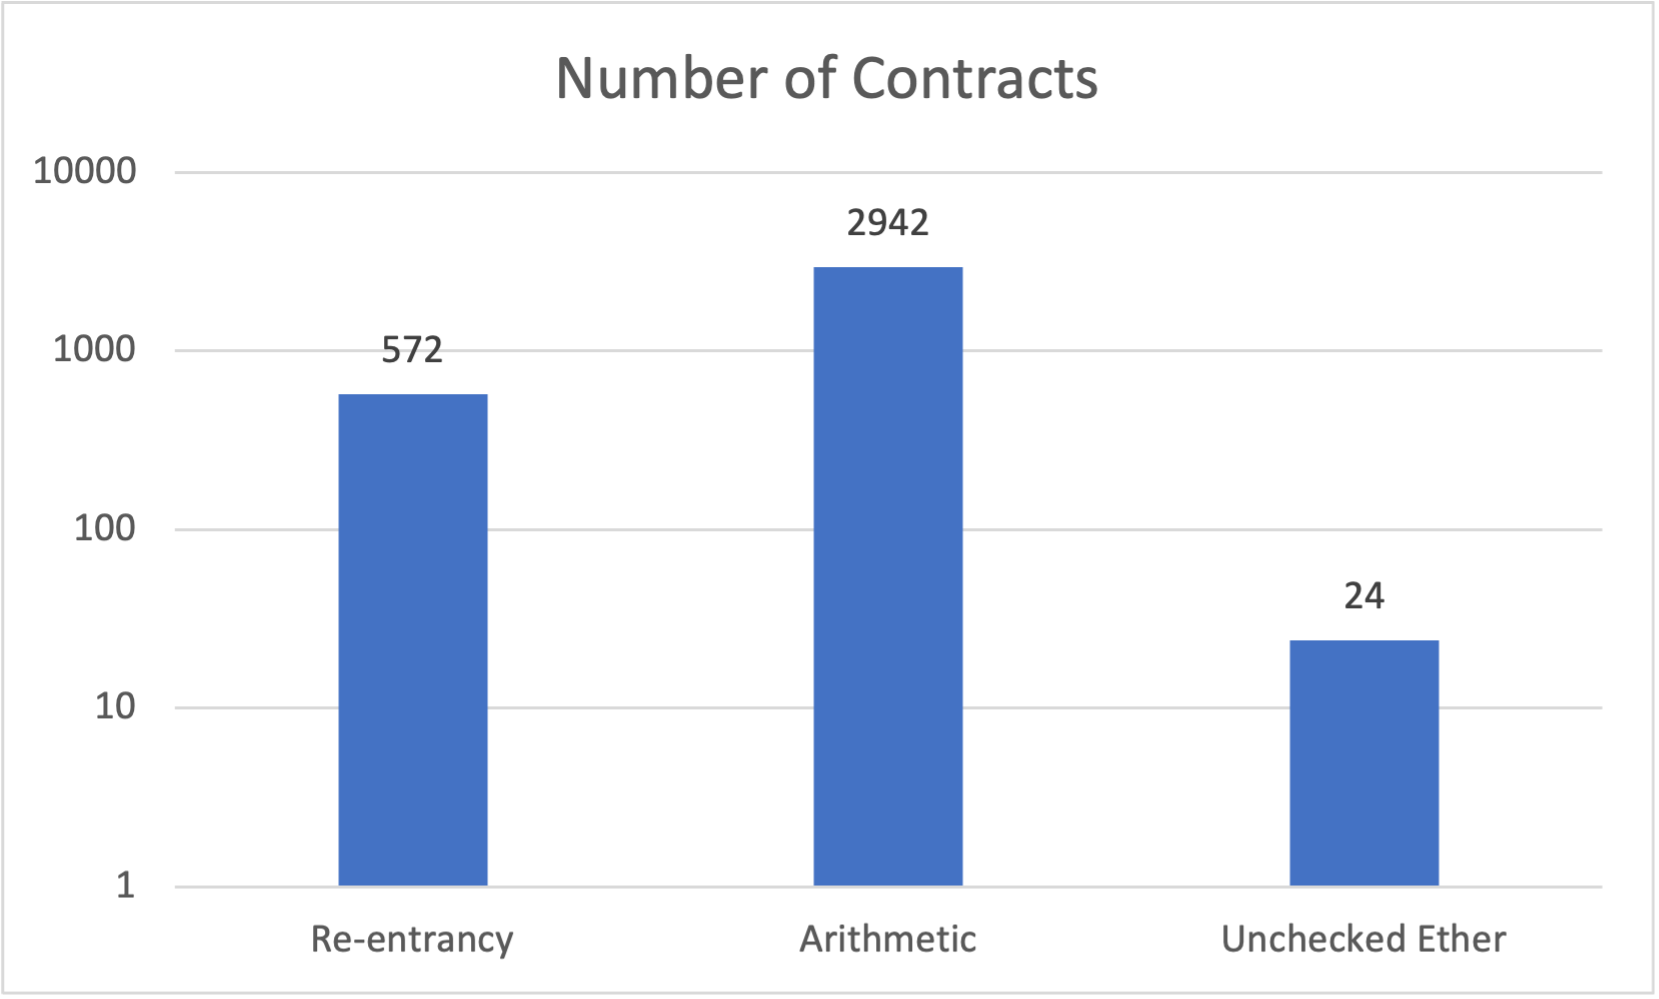
\includegraphics[width=1\textwidth]{figures/Picture1.png}
		\caption{No. of Contracts containing vulnerabilities (log-scale)}
		\label{fig:chart_vuln_count}
	\end{figure}
		
		Figure~\ref{fig:chart_vuln_count} shows the number of smart contracts that contain at least one vulnerability.
		For instance, consider a specific targeted vulnerability.
		The literature tells us that all fo the the three static analyzers in the benchmark support the detection of this vulnerability.
		~\cite{yashavant2022scrawld} notes that they only say the contract at hand contains that vulnerability only if an agreed upon threshold of the tools report that it is present at the same location,
		based on the majority voting system proposed by them. We take on the same system as well for determining wether a vulnerability is present or not.


\section{Concluding Remarks}
	This chapter introduces an up-to-date database, centred around Ethereum smart contracts, namely \etherbase, which includes data on the Ethereum blockchain (blocks),
	its smart contracts, and their metadata.
	Moreover, aggregate statistics and dataset exploration is presented.
	Furthermore, future research directions and opportunities are outlined:

	During the time we were building EtherBase, we utilized Web3 APIs without taking advantage of an Ethereum full / archive node.
	The next version of \etherbase we're already working on, will take full use of an Ethereum full node and instrment it in order to add a variety of more data to EtherBase.
	Collecting data via invoking Web3 API's is very much slower than instrumenting an Ethereum archive node.
	
	In addition, our current method is restricted by the rate limit imposed by the API's.
	For example, Etherescan has a restriction on the daily frequency of queries to its API (5 per day).
	\cite{yashavant2022scrawld} states this as aserious issue which we would like to solve as well.

	We will also be labelling more smart contracts with more tools as we have more time and compute resources moving forward.

	The Ethereum security research community can use \etherbase for evaluating correctness and other parameters of their proposed or other toolsets,
	especially those based on machine learning techniques that need comprhensiver datasets for training, validation, and testing phases.
	\etherbase~comprises a diverse and comprehensive set of real-world heterogenuous annotated smart contracts.
	
	Every tool which was selected for this evaluation is not a complete / sound one, as ~\cite{yashavant2022scrawld} notices this as well.
	There are always many false positive / negatives results in an audit report generated by a static analyser.
	Nevertheless, we utilized the mechanism of majority voting suggested by ~\cite{yashavant2022scrawld}
	to determine the presence or lacke thereof a vulnerability in a smart contract.
	We should, however, be wary of the generated false positive rsults as too many of them will lead to increasing inaccuracies in the released dataset.
	Such issues can be overcome by adding more tools to the benchamrk process or have some auditors manually review the discovered potential vulnerabilities.
	
	Our competitive advantage in comparison to the work done by ~\cite{yashavant2022scrawld} is that \etherbase gets updatedt regularly, is more comprehensive with regards to the various versions of smart contracts it contains,
	and that it leverages offline powerful compialtion tools to retrieve more metadata about the collected smart contracts, instead of going through the time consuming process of validating each collected contract with online services separately and through manual development of data collection pipelines.